\documentclass{article}

% Componentes
\usepackage[utf8]{inputenc} % Codificación de entrada
\usepackage[T1]{fontenc} % Codificación de fuente

\usepackage{amsmath,amsfonts,amssymb} % Paquetes de matemáticas
\usepackage{graphicx} % Para insertar figuras
\usepackage{cite} % Para referencias
\usepackage{hyperref} % Para enlaces

% Título, autores, etc.
\title{Red neuronal 1}
\author{Jorge Butragueño Nieto}
\date{\today}


	

\begin{document}
		\maketitle
	
	\begin{abstract}
		Estudio de una red neuronal sencilla con dos nodos de entrada, dos  nodos ocultos y dos nodos de salida. (ver Figura 1)
	\end{abstract}
	\begin{figure}[h]  % [h] indica que queremos la imagen justo aquí (here)
		\centering    % Centramos la imagen
		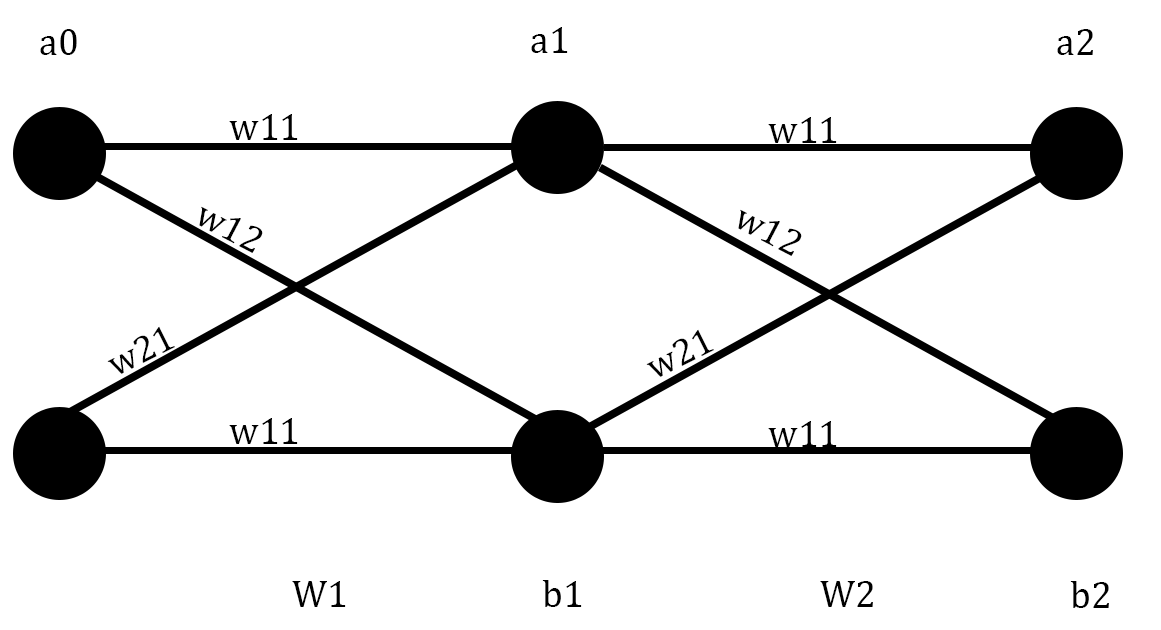
\includegraphics[width=0.5\textwidth]{image.png}  % Especificamos la ruta y el tamaño
		\caption{Red neuronal}  % Añadimos un pie de foto
		\label{fig:ejemplo}  % Etiquetamos la imagen para referenciarla más adelante
	\end{figure}
	\section{Objetivos}
	El objetivo de este estudio será ajustar la red neuronal para que dados unos \textbf{input}, se ajusten todos los pesos y las bias para que devuelva unos \textbf{outputs} muy lo más parecidos a lo deseado y con el menor error posible.
	\section{Inputs y outputs}
	Lo primero será saber qué recibe la red y qué queremos que devuelva. En nuestro caso como recibe dos inputs, y devuelve 2 outputs.
	Construiremos una red que al recibir [1 0] devuelva el contrario es decir, [0 1].
	 \[a^0 = \begin{bmatrix}
	1 & 0
	\end{bmatrix}
	\]
	\[y = \begin{bmatrix}
		0 & 1
	\end{bmatrix}
	\]
	(donde $a^0$ es el input dado, $y$ es el output esperado) \\
	\section{Forward propagation}
	Ahora inicializamos todos los datos que queremos calcular de forma aleatoria y calculamos cuál sería el resultado de la red.
	\subsection{Matrices}
	En el caso de este ejemplo tenemos \(2 \times 2 + 2 \times 2 + 2 + 2 = 12 \) valores que ajustar correctamente, y la mejor forma de organizar todos los cálculos es a través de las matrices.

	\[
	W^1 = \begin{bmatrix}
		w^1_{11} & w^1_{12}  \\
		w^1_{21} & w^1_{22}
	\end{bmatrix}
		W^2 = \begin{bmatrix}
		w^2_{11} & w^2_{12}  \\
		w^2_{21} & w^2_{22}
	\end{bmatrix}
	b^1 = \begin{bmatrix}
		b_1 & b_2
	\end{bmatrix}
		b^2 = \begin{bmatrix}
		b_1 & b_2
	\end{bmatrix}
	\]
	(ver la figura 1)
	\subsection{Calcular el valor de cada nodo}
	A partir de estos valores podemos calcular el valor de cada neurona hasta llegar al final. \\
	Primero con los nodos ocultos:
	\[
	z^1_1 = a^0_1w^1_{11} + a^0_2w^1_{21} + b^1_1 \qquad
	a^1_1 = \sigma (z^2_1)
	\]
	\[
	z^1_2 = a^0_1w^1_{12} + a^0_2w^1_{22} + b^1_1 \qquad
	a^1_2 = \sigma (z^2_2)
	\]
	Finalmente con el output:\\
	\[
	z^2_1 = a^1_1w^2_{11} + a^1_2w^2_{21} + b^2_1 \qquad
	a^2_1 = \sigma (z^2_1)
	\]
	\[
	z^2_2 = a^1_1w^2_{12} + a^1_2w^2_{22} + b^2_1 \qquad
	a^2_2 = \sigma (z^2_2)
	\]
	Nótese que podemos reescribir las anteriores en términos matriciales:
	\[
	Z^1 = a^0 W^1 + b^1
	\]
	\[
	z^1 = 	\begin{bmatrix}
		z^1_1 & z^1_2
	\end{bmatrix} = \begin{bmatrix}
		a^0_1 & a^0_2
	\end{bmatrix} 
	\begin{bmatrix}
		w^1_{11} & w^1_{12}  \\
		w^1_{21} & w^1_{22}
	\end{bmatrix}
	+ 
\begin{bmatrix}
		b^1_1 & b^1_2
	\end{bmatrix} = 
	\begin{bmatrix}
		a^0_1w^1_{11} + a^0_2w^1_{21} + b^1_1 & a^0_1w^1_{12} + a^0_2w^1_{22} + b^1_1
	\end{bmatrix} 
	\]
	\[
Z^2 = a^1 W^2 + b^2
\]
\[
z^2 = 	\begin{bmatrix}
	z^2_1 & z^2_2
\end{bmatrix} = \begin{bmatrix}
	a^1_1 & a^1_2
\end{bmatrix} 
\begin{bmatrix}
	w^2_{11} & w^2_{12}  \\
	w^2_{21} & w^2_{22}
\end{bmatrix}
+ 
\begin{bmatrix}
	b^2_1 & b^2_2
\end{bmatrix} = 
\begin{bmatrix}
	a^1_1w^2_{11} + a^1_2w^2_{21} + b^2_1 & a^1_1w^2_{12} + a^1_2w^2_{22} + b^2_1
\end{bmatrix} 
\]
y finalmente:
\[
a^1 = \sigma(z^1) = \begin{bmatrix}
	\sigma(z^1_1) & \sigma(z^1_2)
\end{bmatrix} 
\]
\[
a^2 = \sigma(z^2) = \begin{bmatrix}
	\sigma(z^2_1) & \sigma(z^2_2)
\end{bmatrix} 
\]
\subsection{Error}
Finalmente una medida para saber cómo de bien está el resultado dado es utilizando el error cuadrático medio MSE
\[
MSE = \frac{1}{n} \sum_{0}^{n} (y_i - \hat{y}_i )
\]
En nuestro caso \( \hat{y} = a^2\) y \(n = 2\) por lo que la función de Coste (C) quedaría:
\[
C = \frac{1}{2} (y_1 - a^2_1)^2 + (y_2 - a^2_2)^2
\]

\section{Backpropagation}
\subsection{Cálculo del gradiente}
Para poder reducir al máximo el error usaremos el descenso por gradiente, donde será necesario calcular el gradiente de nuestra función.
El gradiente se obtiene como la derivada de cada una de nuestras variables, en nuestro caso son 12:
\[
\frac{\partial C}{\partial W^2} = \scalebox{1}{$
	\begin{bmatrix}
		\frac{\partial C}{\partial w^2_{11}} & \frac{\partial C}{\partial w^2_{12}} \\
		\frac{\partial C}{\partial w^2_{21}} & \frac{\partial C}{\partial w^2_{22}}
	\end{bmatrix}$
}
\frac{\partial C}{\partial W^1} = \scalebox{1}{$
	\begin{bmatrix}
		\frac{\partial C}{\partial w^1_{11}} & \frac{\partial C}{\partial w^1_{12}} \\
		\frac{\partial C}{\partial w^1_{21}} & \frac{\partial C}{\partial w^1_{22}}
	\end{bmatrix}$
}
\]
\[
\frac{\partial C}{\partial b^2} = \scalebox{1}{$
	\begin{bmatrix}
		\frac{\partial C}{\partial b^2_1} & \frac{\partial C}{\partial b^2_2} 
	\end{bmatrix}$
}
\frac{\partial C}{\partial b^1} = \scalebox{1}{$
	\begin{bmatrix}
		\frac{\partial C}{\partial b^1_1} & \frac{\partial C}{\partial b^1_2} 
	\end{bmatrix}$
}
\]
Para calcular las derivadas haremos uso de la regla de la cadena
\[
\frac{\partial C} {\partial W^2} =  \scalebox{1}{$ \begin{bmatrix}
	\frac{\partial C}{\partial a^2_1} \frac{\partial  a^2_1}{\partial z^2_1} \frac{\partial z^2_1 }{\partial w^2_{11}} &
	\frac{\partial C}{\partial a^2_2} \frac{\partial  a^2_2}{\partial z^2_2} \frac{\partial z^2_2}{\partial w^2_{12}} \\
	\frac{\partial C}{\partial a^2_1} \frac{\partial  a^2_1}{\partial z^2_1} \frac{\partial z^2_1}{\partial w^2_{21}}  & 
	\frac{\partial C}{\partial a^2_2} \frac{\partial  a^2_2}{\partial z^2_2} \frac{\partial z^2_2}{\partial w^2_{22}}
\end{bmatrix}$}
\]
\[
\frac{\partial C} {\partial b^2} =  \scalebox{1.}{$ \begin{bmatrix}
		\frac{\partial C}{\partial a^2_1} \frac{\partial  a^2_1}{\partial z^2_1} \frac{\partial z^2_1 }{\partial b^2_{1}} &
		\frac{\partial C}{\partial a^2_2} \frac{\partial  a^2_2}{\partial z^2_2} \frac{\partial z^2_2}{\partial b^2_{2}} 
	\end{bmatrix}$}
\]

\[
\frac{\partial C} {\partial W^1} =  \scalebox{1}{$ \begin{bmatrix}
		\frac{\partial C}{\partial a^2_1} \frac{\partial  a^2_1}{\partial z^2_1} \frac{\partial z^2_1 }{\partial a^1_{1}} \frac{\partial a^1_1}{\partial z^1_1} \frac{\partial z^1_1 }{\partial w^1_{11}} +  \frac{\partial C}{\partial a^2_2} \frac{\partial  a^2_2}{\partial z^2_2} \frac{\partial z^2_2 }{\partial a^1_{1}} \frac{\partial a^1_1}{\partial z^1_1} \frac{\partial z^1_1 }{\partial w^1_{11}}
		&
		\frac{\partial C}{\partial a^2_1} \frac{\partial  a^2_1}{\partial z^2_1} \frac{\partial z^2_1 }{\partial a^1_{2}} \frac{\partial a^1_2}{\partial z^1_2} \frac{\partial z^1_2 }{\partial w^1_{12}} +  \frac{\partial C}{\partial a^2_2} \frac{\partial  a^2_2}{\partial z^2_2} \frac{\partial z^2_2 }{\partial a^1_{2}} \frac{\partial a^1_2}{\partial z^1_2} \frac{\partial z^1_2 }{\partial w^1_{12}}
		\\
		\frac{\partial C}{\partial a^2_1} \frac{\partial  a^2_1}{\partial z^2_1} \frac{\partial z^2_1 }{\partial a^1_{1}} \frac{\partial a^1_1}{\partial z^1_1} \frac{\partial z^1_1 }{\partial w^1_{21}} +  \frac{\partial C}{\partial a^2_2} \frac{\partial  a^2_2}{\partial z^2_2} \frac{\partial z^2_2 }{\partial a^1_{1}} \frac{\partial a^1_1}{\partial z^1_1} \frac{\partial z^1_1 }{\partial w^1_{21}}
		& 
		\frac{\partial C}{\partial a^2_1} \frac{\partial  a^2_1}{\partial z^2_1} \frac{\partial z^2_1 }{\partial a^1_{2}} \frac{\partial a^1_2}{\partial z^1_2} \frac{\partial z^1_2 }{\partial w^1_{22}} +  \frac{\partial C}{\partial a^2_2} \frac{\partial  a^2_2}{\partial z^2_2} \frac{\partial z^2_2 }{\partial a^1_{2}} \frac{\partial a^1_2}{\partial z^1_2} \frac{\partial z^1_2 }{\partial w^1_{22}}
	\end{bmatrix}$}
\]
\[
\frac{\partial C} {\partial b^1} =  \scalebox{1}{$ \begin{bmatrix}
		\frac{\partial C}{\partial a^2_1} \frac{\partial  a^2_1}{\partial z^2_1} \frac{\partial z^2_1 }{\partial a^1_{1}} \frac{\partial a^1_1}{\partial z^1_1} \frac{\partial z^1_1 }{\partial b^1_{1}} + \frac{\partial C}{\partial a^2_2} \frac{\partial  a^2_2}{\partial z^2_2} \frac{\partial z^2_2 }{\partial a^1_{1}} \frac{\partial a^1_1}{\partial z^1_1} \frac{\partial z^1_1 }{\partial b^1_{1}}
		&
		\frac{\partial C}{\partial a^2_1} \frac{\partial  a^2_1}{\partial z^2_1} \frac{\partial z^2_1 }{\partial a^1_{2}} \frac{\partial a^1_2}{\partial z^1_2} \frac{\partial z^1_2 }{\partial b^1_{2}} +  \frac{\partial C}{\partial a^2_2} \frac{\partial  a^2_2}{\partial z^2_2} \frac{\partial z^2_2 }{\partial a^1_{2}} \frac{\partial a^1_2}{\partial z^1_2} \frac{\partial z^1_2 }{\partial b^1_{2}}

	\end{bmatrix}$}
\]


	% Actualización de los pesos usando descenso por gradiente
	\section{Descenso por Gradiente}
	
	La actualización de los pesos \( w_{ij} \) y los biases \( b_j \) en una red neuronal utilizando descenso por gradiente se realiza de la siguiente manera:
	
	\subsection*{Actualización de los Pesos}
	
	\begin{equation}
		w_{ij}^{(t+1)} = w_{ij}^{(t)} - \eta \frac{\partial C}{\partial w_{ij}}
	\end{equation}
	
	\subsection*{Actualización de los Biases}
	
	\begin{equation}
		b_j^{(t+1)} = b_j^{(t)} - \eta \frac{\partial C}{\partial b_j}
	\end{equation}
	
	\subsection*{Versión Combinada}
	
	Si consideramos todos los pesos \( \mathbf{W} \) y biases \( \mathbf{b} \):
	
	\begin{equation}
		\mathbf{W}^{(t+1)} = \mathbf{W}^{(t)} - \eta \nabla_{\mathbf{W}} C
	\end{equation}
	
	\begin{equation}
		\mathbf{b}^{(t+1)} = \mathbf{b}^{(t)} - \eta \nabla_{\mathbf{b}} C
	\end{equation}
	





	
	
\end{document}
